% Created by tikzDevice version 0.8.1 on 2015-02-22 23:14:01
% !TEX encoding = UTF-8 Unicode
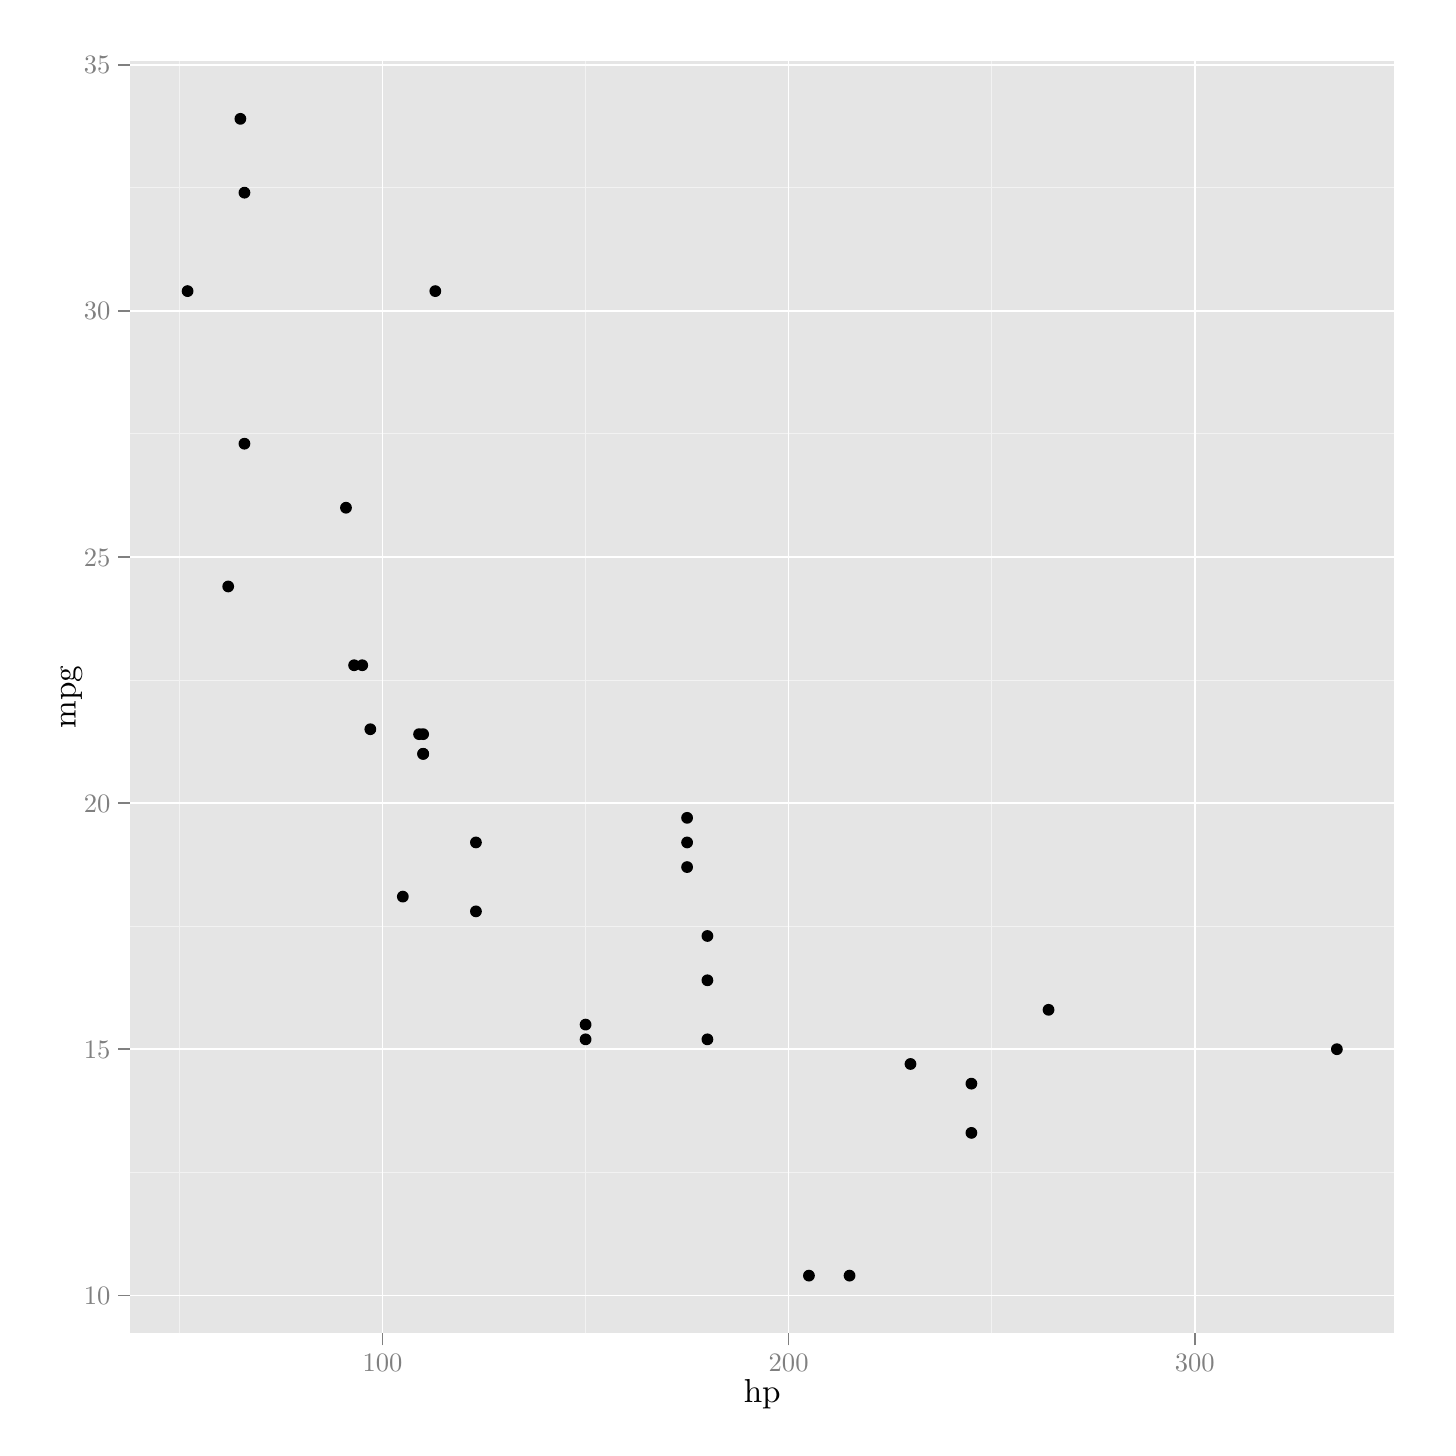
\begin{tikzpicture}[x=1pt,y=1pt]
\definecolor{fillColor}{RGB}{255,255,255}
\path[use as bounding box,fill=fillColor,fill opacity=0.00] (0,0) rectangle (505.89,505.89);
\begin{scope}
\path[clip] (  0.00,  0.00) rectangle (505.89,505.89);
\definecolor{drawColor}{RGB}{255,255,255}
\definecolor{fillColor}{RGB}{255,255,255}

\path[draw=drawColor,line width= 0.6pt,line join=round,line cap=round,fill=fillColor] (  0.00,  0.00) rectangle (505.89,505.89);
\end{scope}
\begin{scope}
\path[clip] ( 37.02, 34.03) rectangle (493.85,493.85);
\definecolor{fillColor}{gray}{0.90}

\path[fill=fillColor] ( 37.02, 34.03) rectangle (493.85,493.85);
\definecolor{drawColor}{gray}{0.95}

\path[draw=drawColor,line width= 0.3pt,line join=round] ( 37.02, 92.29) --
	(493.85, 92.29);

\path[draw=drawColor,line width= 0.3pt,line join=round] ( 37.02,181.23) --
	(493.85,181.23);

\path[draw=drawColor,line width= 0.3pt,line join=round] ( 37.02,270.17) --
	(493.85,270.17);

\path[draw=drawColor,line width= 0.3pt,line join=round] ( 37.02,359.10) --
	(493.85,359.10);

\path[draw=drawColor,line width= 0.3pt,line join=round] ( 37.02,448.04) --
	(493.85,448.04);

\path[draw=drawColor,line width= 0.3pt,line join=round] ( 54.85, 34.03) --
	( 54.85,493.85);

\path[draw=drawColor,line width= 0.3pt,line join=round] (201.60, 34.03) --
	(201.60,493.85);

\path[draw=drawColor,line width= 0.3pt,line join=round] (348.35, 34.03) --
	(348.35,493.85);
\definecolor{drawColor}{RGB}{255,255,255}

\path[draw=drawColor,line width= 0.6pt,line join=round] ( 37.02, 47.82) --
	(493.85, 47.82);

\path[draw=drawColor,line width= 0.6pt,line join=round] ( 37.02,136.76) --
	(493.85,136.76);

\path[draw=drawColor,line width= 0.6pt,line join=round] ( 37.02,225.70) --
	(493.85,225.70);

\path[draw=drawColor,line width= 0.6pt,line join=round] ( 37.02,314.63) --
	(493.85,314.63);

\path[draw=drawColor,line width= 0.6pt,line join=round] ( 37.02,403.57) --
	(493.85,403.57);

\path[draw=drawColor,line width= 0.6pt,line join=round] ( 37.02,492.51) --
	(493.85,492.51);

\path[draw=drawColor,line width= 0.6pt,line join=round] (128.22, 34.03) --
	(128.22,493.85);

\path[draw=drawColor,line width= 0.6pt,line join=round] (274.97, 34.03) --
	(274.97,493.85);

\path[draw=drawColor,line width= 0.6pt,line join=round] (421.72, 34.03) --
	(421.72,493.85);
\definecolor{fillColor}{RGB}{0,0,0}

\path[fill=fillColor] (142.90,243.48) circle (  2.13);

\path[fill=fillColor] (142.90,243.48) circle (  2.13);

\path[fill=fillColor] (117.95,275.50) circle (  2.13);

\path[fill=fillColor] (142.90,250.60) circle (  2.13);

\path[fill=fillColor] (238.28,202.57) circle (  2.13);

\path[fill=fillColor] (135.56,191.90) circle (  2.13);

\path[fill=fillColor] (341.01,124.31) circle (  2.13);

\path[fill=fillColor] ( 72.46,303.96) circle (  2.13);

\path[fill=fillColor] (120.89,275.50) circle (  2.13);

\path[fill=fillColor] (161.98,211.47) circle (  2.13);

\path[fill=fillColor] (161.98,186.56) circle (  2.13);

\path[fill=fillColor] (245.62,161.66) circle (  2.13);

\path[fill=fillColor] (245.62,177.67) circle (  2.13);

\path[fill=fillColor] (245.62,140.32) circle (  2.13);

\path[fill=fillColor] (282.31, 54.94) circle (  2.13);

\path[fill=fillColor] (296.98, 54.94) circle (  2.13);

\path[fill=fillColor] (319.00,131.42) circle (  2.13);

\path[fill=fillColor] ( 78.33,446.26) circle (  2.13);

\path[fill=fillColor] ( 57.79,410.69) circle (  2.13);

\path[fill=fillColor] ( 76.86,472.94) circle (  2.13);

\path[fill=fillColor] (123.82,252.38) circle (  2.13);

\path[fill=fillColor] (201.60,145.65) circle (  2.13);

\path[fill=fillColor] (201.60,140.32) circle (  2.13);

\path[fill=fillColor] (341.01,106.52) circle (  2.13);

\path[fill=fillColor] (238.28,211.47) circle (  2.13);

\path[fill=fillColor] ( 78.33,355.55) circle (  2.13);

\path[fill=fillColor] (115.02,332.42) circle (  2.13);

\path[fill=fillColor] (147.30,410.69) circle (  2.13);

\path[fill=fillColor] (368.89,150.99) circle (  2.13);

\path[fill=fillColor] (238.28,220.36) circle (  2.13);

\path[fill=fillColor] (473.08,136.76) circle (  2.13);

\path[fill=fillColor] (141.43,250.60) circle (  2.13);
\end{scope}
\begin{scope}
\path[clip] (  0.00,  0.00) rectangle (505.89,505.89);
\definecolor{drawColor}{gray}{0.50}

\node[text=drawColor,anchor=base east,inner sep=0pt, outer sep=0pt, scale=  0.96] at ( 29.91, 44.51) {10};

\node[text=drawColor,anchor=base east,inner sep=0pt, outer sep=0pt, scale=  0.96] at ( 29.91,133.45) {15};

\node[text=drawColor,anchor=base east,inner sep=0pt, outer sep=0pt, scale=  0.96] at ( 29.91,222.39) {20};

\node[text=drawColor,anchor=base east,inner sep=0pt, outer sep=0pt, scale=  0.96] at ( 29.91,311.33) {25};

\node[text=drawColor,anchor=base east,inner sep=0pt, outer sep=0pt, scale=  0.96] at ( 29.91,400.27) {30};

\node[text=drawColor,anchor=base east,inner sep=0pt, outer sep=0pt, scale=  0.96] at ( 29.91,489.21) {35};
\end{scope}
\begin{scope}
\path[clip] (  0.00,  0.00) rectangle (505.89,505.89);
\definecolor{drawColor}{gray}{0.50}

\path[draw=drawColor,line width= 0.6pt,line join=round] ( 32.75, 47.82) --
	( 37.02, 47.82);

\path[draw=drawColor,line width= 0.6pt,line join=round] ( 32.75,136.76) --
	( 37.02,136.76);

\path[draw=drawColor,line width= 0.6pt,line join=round] ( 32.75,225.70) --
	( 37.02,225.70);

\path[draw=drawColor,line width= 0.6pt,line join=round] ( 32.75,314.63) --
	( 37.02,314.63);

\path[draw=drawColor,line width= 0.6pt,line join=round] ( 32.75,403.57) --
	( 37.02,403.57);

\path[draw=drawColor,line width= 0.6pt,line join=round] ( 32.75,492.51) --
	( 37.02,492.51);
\end{scope}
\begin{scope}
\path[clip] (  0.00,  0.00) rectangle (505.89,505.89);
\definecolor{drawColor}{gray}{0.50}

\path[draw=drawColor,line width= 0.6pt,line join=round] (128.22, 29.77) --
	(128.22, 34.03);

\path[draw=drawColor,line width= 0.6pt,line join=round] (274.97, 29.77) --
	(274.97, 34.03);

\path[draw=drawColor,line width= 0.6pt,line join=round] (421.72, 29.77) --
	(421.72, 34.03);
\end{scope}
\begin{scope}
\path[clip] (  0.00,  0.00) rectangle (505.89,505.89);
\definecolor{drawColor}{gray}{0.50}

\node[text=drawColor,anchor=base,inner sep=0pt, outer sep=0pt, scale=  0.96] at (128.22, 20.31) {100};

\node[text=drawColor,anchor=base,inner sep=0pt, outer sep=0pt, scale=  0.96] at (274.97, 20.31) {200};

\node[text=drawColor,anchor=base,inner sep=0pt, outer sep=0pt, scale=  0.96] at (421.72, 20.31) {300};
\end{scope}
\begin{scope}
\path[clip] (  0.00,  0.00) rectangle (505.89,505.89);
\definecolor{drawColor}{RGB}{0,0,0}

\node[text=drawColor,anchor=base,inner sep=0pt, outer sep=0pt, scale=  1.20] at (265.43,  9.03) {hp};
\end{scope}
\begin{scope}
\path[clip] (  0.00,  0.00) rectangle (505.89,505.89);
\definecolor{drawColor}{RGB}{0,0,0}

\node[text=drawColor,rotate= 90.00,anchor=base,inner sep=0pt, outer sep=0pt, scale=  1.20] at ( 17.30,263.94) {mpg};
\end{scope}
\end{tikzpicture}
